\section{Apéndice}

\subsection{Apéndice I: detalles de implementación}

Para poder soportar la posible necesidad de matrices más eficientes en memoria, creamos una clase Matrix con múltiples implementaciones. La misma tiene métodos para cada operación que consideramos necesaria, y algunas otras utilidades que utilizamos en el Trabajo Práctico 1. Por otro lado, implementamos una matriz completa (con vectores de la biblioteca estándar de C++), una matriz dispersa (usando mapas), y otras versiones más específicas.

Para evitar complicaciones con el manejo de punteros y el polimorfismo, utilizamos \texttt{std::shared\_ptr} de C++11, que se encarga de borrar las matrices que no necesitamos por nosotros.

Sin embargo, luego nos dimos cuenta que los casos de uso de este TP no requieren varias versiones especificas como si las requería tal vez el TP anterior. La implementación sigue incluída, pero solo se usa la versión completa de la matriz (denominada \texttt{FullMatrix}).

Otro elemento que dejamos en la implementación pero no se utiliza fueron unos pseudo-iteradores para las imágenes que recorren archivos en lugar de vectores en memoria. El mismo no se usa porque es muy poco eficiente (ya que lee múltiples veces un archivo en disco), y luego de medir el consumo de memoria lo consideramos innecesario.

Por otro lado, decidimos abstraer el entrenamiento y el reconocimiento de las imágenes en una clase común, a modo de intercambiar implemetaciones rápidamente y por parámetros. Hoy en día nuestro TP solo cuenta con 2 implementaciones: kNN y kNN + PCA, pero podrían argegarse otras variaciones a futuro.

\subsection{Apéndice II: código complementario en MATLAB}

Además del código con el reconocimiento de dígitos implementado en C++, incluímos en la entrega algunos scripts de MATLAB que nos resultaron útiles durante la experimentación. Los mismos incluyen comentarios explicando su funcionalidad, pero todos están relacionados a los datos con los que expermientamos (con algunos métodos para probar incrementando el set de entrenamiento) y los resultados de dichos experimentos (validación cruzada, F1 score, etc).

\subsection{Apéndice III: Gráficos e imágenes}

\begin{figure}[H]
    \begin{center}
      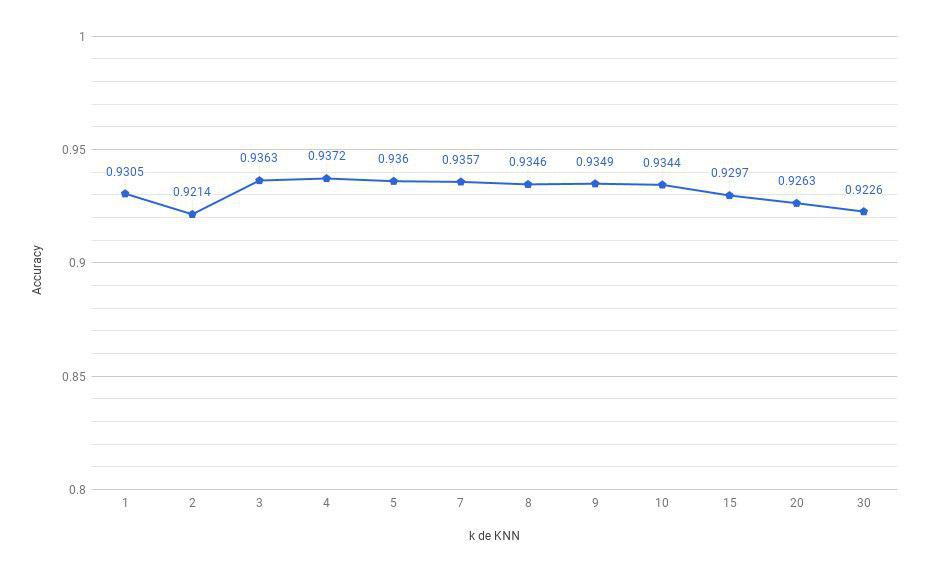
\includegraphics[width=0.8\columnwidth]{imagenes/knn-accuracy.jpg}
      \caption{Accuracy por k de kNN}
    \end{center}
\end{figure}

\begin{figure}[H]
    \begin{center}
      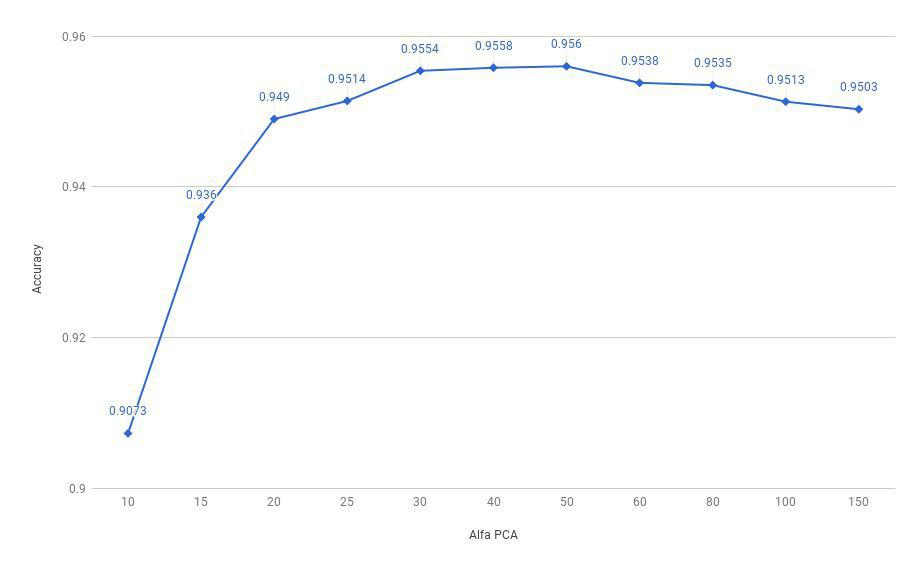
\includegraphics[width=0.8\columnwidth]{imagenes/pca-accuracy.jpg}
      \caption{Accuracy por alfa de PCA}
    \end{center}
\end{figure}

\begin{figure}[H]
    \begin{center}
      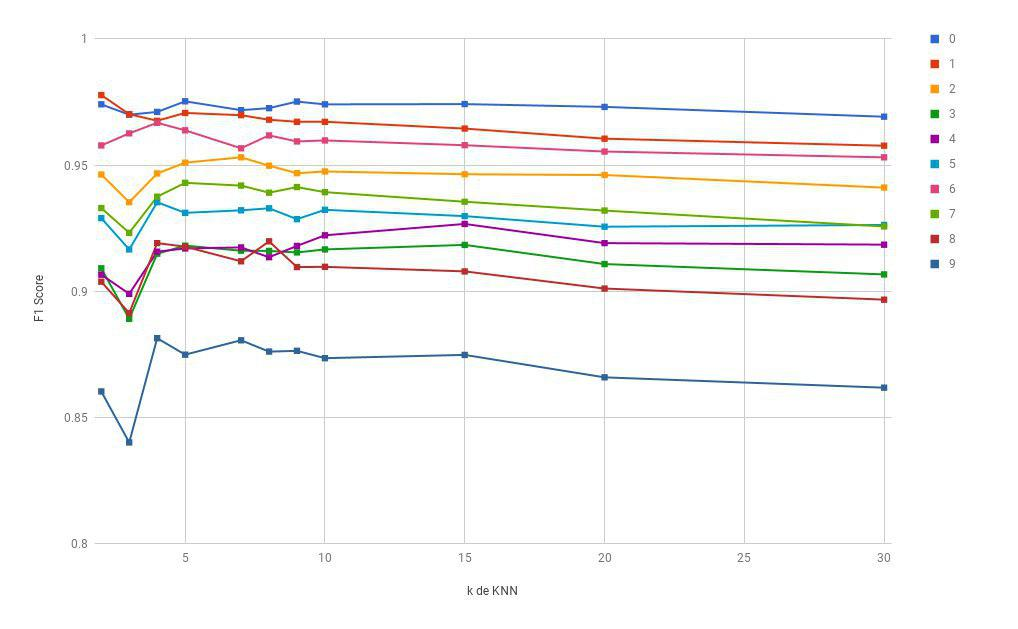
\includegraphics[width=0.8\columnwidth]{imagenes/knn-f1.jpg}
      \caption{F1 Score por k de kNN}
    \end{center}
\end{figure}

\begin{figure}[H]
    \begin{center}
      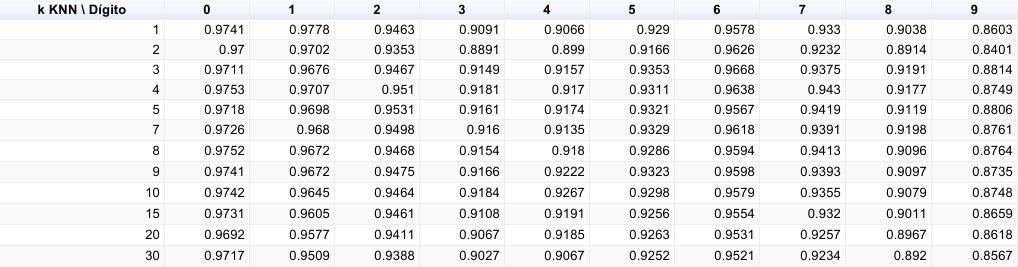
\includegraphics[width=0.8\columnwidth]{imagenes/knn-f1-table.jpg}
      \caption{F1 Score por k de kNN}
    \end{center}
\end{figure}

\begin{figure}[H]
    \begin{center}
      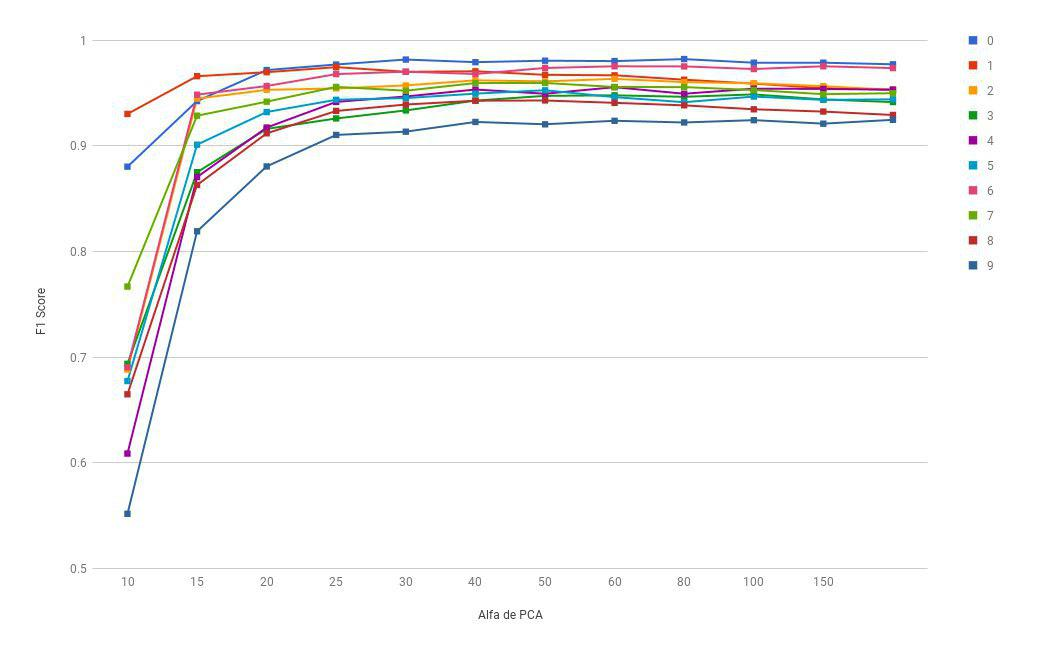
\includegraphics[width=0.8\columnwidth]{imagenes/pca-f1.jpg}
      \caption{F1 Score por alfa de PCA}
    \end{center}
\end{figure}

\begin{figure}[H]
    \begin{center}
      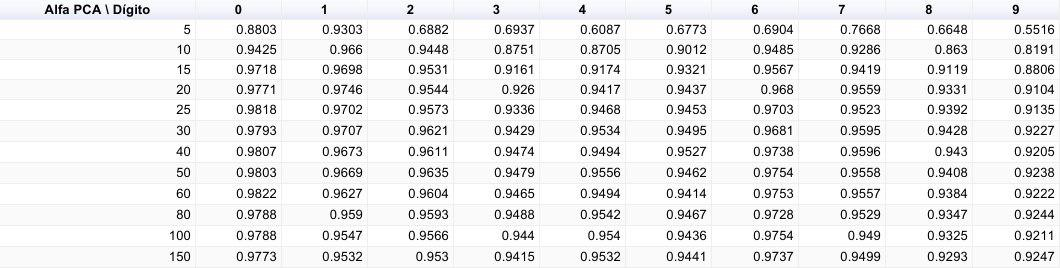
\includegraphics[width=0.8\columnwidth]{imagenes/pca-f1-table.jpg}
      \caption{F1 Score por alfa de PCA}
    \end{center}
\end{figure}